\documentclass[aspectratio=169]{beamer}

\mode<presentation>

\usepackage[utf8]{inputenc}
\usepackage[T1]{fontenc}
\usepackage{amsmath}
\usepackage{graphicx}
\usepackage{hyperref}
\usepackage{listings}
\usepackage{xcolor}
\usepackage{multicol}


\usepackage[swedish]{babel}

\usepackage{../../../Common/mau}


\lstset{style=java}

\title{DA102A---F4: Klassdiagram}
\author{Malmö universitet}
\date{2025--??--??}

\institute{Institutionen för datavetenskap och medieteknik}

\begin{document}

\begin{frame}
    \frametitle{Innehåll}

    \textbox{\tableofcontents}

\end{frame}

\section{Repetition}

\begin{frame}
    \frametitle{Repetition}
    \framesubtitle{Klasser}

    \textbox{En klass var en mall för att skapa objekt.}

    \textbox{Objekt hade attribut och operationer. (Variabler och metoder)}

    \textbox{Vi kunde skapa flera objekt av samma klass.}

\end{frame}

\begin{frame}[fragile]
    \frametitle{Repetition}
    \framesubtitle{Klasser, exempel}

    \begin{lstlisting}
public class Person{
    private String name; // Attribut
    public Person(){ // Default konstruktor
        this.Person("Ingen"); // Vi anropar den andra konstruktorn
    }
    public Person(String n){ // Konstruktor
        this.name = n; // Kom ihåg this
    }
    public String greeting(){ // Operation
        return "My name is " + this.name;
    }
}
    \end{lstlisting}

\end{frame}

\begin{frame}[fragile]
    \frametitle{Repetition}
    \framesubtitle{Klasser, exempel}

    \begin{lstlisting}
// Initialiserar nya instanser av Person
Person teacher1 = new Person("Sebastian");
Person teacher2 = new Person("Calle");
Person teacher3 = new Person(); 
// Anropar de olika instansernas greeting
System.out.println(teacher1.greeting());
System.out.println(teacher2.greeting());
System.out.println(teacher3.greeting());
    \end{lstlisting}
\end{frame}

\section{Klassdiagram}

\begin{frame}
    \frametitle{Klassdiagram}
    \framesubtitle{Varför använda klassdiagram}

    \textbox{När du ska prata med din boomer chef}

    \textbox{Ger en blueprint på hur en klass ska byggas upp}

    \textbox{Kommunicera din implementation med andra}

\end{frame}

\begin{frame}[fragile]
    \frametitle{Klassdiagram}
    \framesubtitle{Exempel, en klass}

    \begin{lstlisting}
public class Person{
    private String name; // Attribut
    private int birthYear; // Ett till attribut
    public Person(){ // Default konstruktor
        this.Person("Ingen",2025); // Vi anropar den andra konstruktorn
    }
    public Person(String n, int y){ // Konstruktor
        this.name = n; // Kom ihåg this
        this.birthYear = y;
    }
    public String greeting(){ // Operation
        return "My name is " + this.name;
    }
}
    \end{lstlisting}

\end{frame}

\begin{frame}
    \frametitle{Klassdiagram}
    \framesubtitle{Exempel, ett klassdiagram}

    \centering
    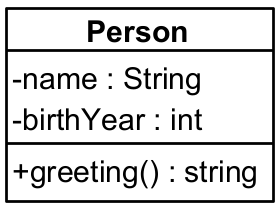
\includegraphics[]{person.png}

\end{frame}

\begin{frame}
    \frametitle{Klassdiagram}
    \framesubtitle{}

    \textbox{Översta rutan: Klassnamn}

    \textbox{Mellersta rutan: Attribut (variabler)}

    \textbox{Nedersta rutan: Operationer (metoder)}

\end{frame}

\begin{frame}[fragile]
    \frametitle{Klassdiagram}
    \framesubtitle{Större exempel}

    \centering
    

\end{frame}

\section{Relationer}

\section{Sammanfattning}

\begin{frame}
    \frametitle{Rekommenderad läsning}

    \textbox{Dietel \& Dietel}

    \textbox{Scott Lynch, \textit{The Lies of Locke Lamora}}
\end{frame}

\end{document}